\section{Gestor de mensajes}
El \textbf{Message Management} se encarga de gestionar los mensajes que son
enviados y recibidos desde la red CAN. Esta entidad debe ser capaz de determinar
si el mensaje (enviado o recibido) contiene datos o eventos. El gestor de
mensajes tiene cuatro entidades:
\begin{itemize}
\item \textit{Receiver Manager}: es el encargado de recibir los mansajes de la
  capa inferior a traves de la interfaz NMT. Esta entidad recibe y despaquetiza
  los mensajes.
\item \textit{Prepared Message}: es el encargado de recibir los mensajes desde
  las capas superiores para ser enviado a la red.
\item \textit{Sorter Message}: es el encargado de clasificar los mensajes,
  ya sea aquellos que envía a la red CAN comos los que recibe de esta. Su
  principal función es verificar  el tipo de mensaje que está recibiendo o
  enviando (datos o eventos). Los eventos tiene mayor prioridad que los datos
  y deben atenderse con urgencia.
\item \textit{Buffer Message}: este sirve de buffer para almacenar mensajes
  tanto que se envían como lo que se reciben. Este buffer es utilizado por el
  \textit{Sorter Message}.
\end{itemize}

\todo[inline]{AGREGAR IMAGEN}
\begin{figure}[h!]
 \centering
 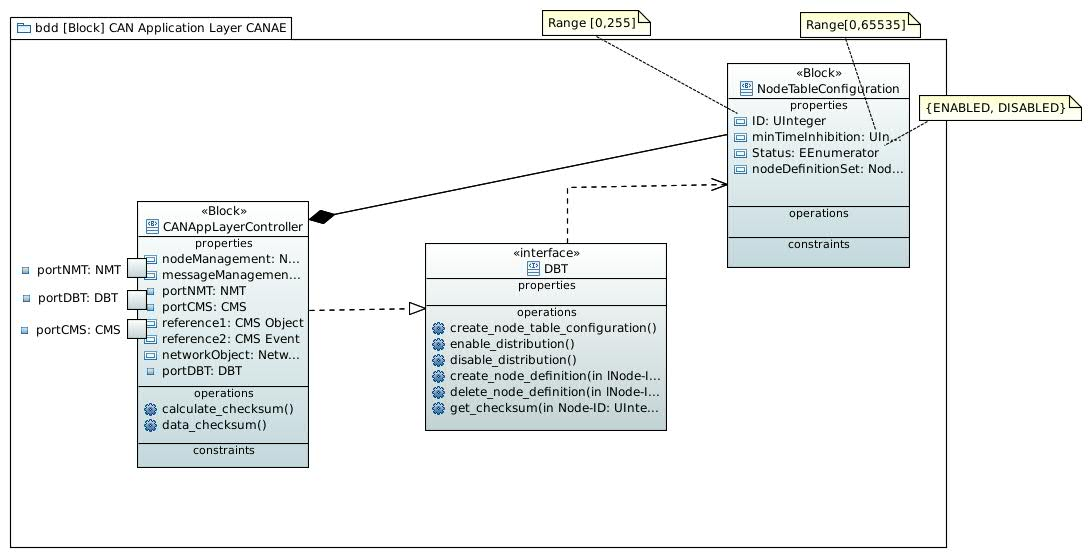
\includegraphics[scale=0.4]{images/Secciones/AppendixA/DBT.JPG}
  \caption{Arquitectura de la entidad DBT}
\label{fig:DBT}
\end{figure}


\subsection{Receiver Manager}
Esta entidad perteneciente al \textit{Message Management} se encarga de recibir
los mensajes de la capa inmediatamente inferior a través de la interfaz NMT (y
sus protocolos). Esta entidad recibe y despaquetiza los paquetes. Se supone que
los mensajes llegan sin ningún tipo de error.

Las principales funciones de esta entidad son las siguientes:
\begin{itemize}
\item receive\_message(Message message): esta es la operación que se debe llamar
  para recibir el mensaje proveniente de la capa inferior. 
  \begin{itemize}
  \item \textbf{Data message}: Es el mensaje que recibe de las capas inferiores
    de la red CAN.
  \end{itemize}
\end{itemize}

\subsection{Sorter Message}
Esta entidad es el encargado de clasificar los mensajes que provienen tanto del
\textit{Receiver Message} y \textit{Prepared Message}. Este clasifica los
mensajes recibidos o por enviar, de modo tal de conocer aquellos que sean
datos o eventos. Debe tenerse en cuenta que los eventos tiene mayor prioridad
que los datos, debido a que (en su mayoría) informan de algún problema a la red.

Las principales funciones con las que cuenta esta entidad son las siguiente:
\begin{itemize}
  \item Boolean extract\_type\_message(Data message): esta operación permite
  extraer el tipo de información que contiene el mensaje: datos o evento.
  \begin{itemize}
  \item \textbf{Data message}: es el mensaje que recibe de las capas inferiores
    de la red CAN.
  \item \textbf{Return Boolean}: retorna 1 se se trata de un evento, 0 si se
    trata de un dato.
  \end{itemize}

\item Boolean send\_message(Message message): esta función envía los mensajes
  a las capas inferiores a través del protocol NMT.
  \begin{itemize}
  \item \textbf{Message message}: es el mensaje formateado listo para enviar.
  \item \textbf{Return Boolean}: retorna 1 si la operación se llevó
    correctamente.
  \end{itemize}
\item Boolean send\_event(Message message): esta función envía el evento en
  forma de mensajes formateado. 
    \begin{itemize}
  \item \textbf{Message message}: es el mensaje formateado listo para enviar.
  \item \textbf{Return Boolean}: retorna 1 si la operación se llevó
    correctamente.
  \end{itemize}
\end{itemize}


\subsection{Buffer Messages}
Esta es la entidad que permite almacenar los mensajes que son recibidos y
enviados. Esta entidad debe controlar la integridad de los mensajes que se
encuentran almacenados. Además se encarga de escribir y leer los mensajes
almacenados en el buffer. El buffer es FIFO\footnote{First In First Out}.

Las principales funciones de esta entidad son las siguientes:
\begin{itemize}
\item save\_message(Message message): esta función almacena el mensaje en
  el buffer de mensajes
  \begin{itemize}
  \item \textbf{Message message}: es el mensaje formateado listo para enviar.
  \end{itemize}
  
\item Message read\_last\_message(): esta función lee el último mensaje.
  \begin{itemize}
    \item \textbf{Return Message}: retorna el mensaje extraído del buffer.
  \end{itemize}
  
\end{itemize}






